% coding:utf-8

%kugprg, a LaTeX-Code for a summary of programming modules
%Copyright (C) 2013, Daniel Winz, Ervin Mazlagic

%This program is free software; you can redistribute it and/or
%modify it under the terms of the GNU General Public License
%as published by the Free Software Foundation; either version 2
%of the License, or (at your option) any later version.

%This program is distributed in the hope that it will be useful,
%but WITHOUT ANY WARRANTY; without even the implied warranty of
%MERCHANTABILITY or FITNESS FOR A PARTICULAR PURPOSE.  See the
%GNU General Public License for more details.
%----------------------------------------

\documentclass[a4paper,10pt,fleqn]{article}

\usepackage{layout}

\title{Zusammenfassung Programmieren und Algorithmen}

\author{Daniel Winz\\Ervin Mazlagi\'c}
\date{\today~\dtc}


\begin{document}

\maketitle

% coding:utf-8

%kugprg, a LaTeX-Code for a summary of programming modules
%Copyright (C) 2013, Daniel Winz, Ervin Mazlagic

%This program is free software; you can redistribute it and/or
%modify it under the terms of the GNU General Public License
%as published by the Free Software Foundation; either version 2
%of the License, or (at your option) any later version.

%This program is distributed in the hope that it will be useful,
%but WITHOUT ANY WARRANTY; without even the implied warranty of
%MERCHANTABILITY or FITNESS FOR A PARTICULAR PURPOSE.  See the
%GNU General Public License for more details.
%----------------------------------------

\chapter*{Über diese Arbeit}
Dies ist das Ergebnis einer Zusammenarbeit auf Basis freier Texte erstellt von 
Studierenden der Fachhochschule Luzern und ist unter der GPLv2 lizenziert. Der 
\TeX - bzw. \LaTeX -Code ist auf \url{github.com/fosa/fosaet} hinterlegt.Eine 
aktuelle PDF-Ausgabe steht auf \url{fosa.adinox.ch} zum Download bereit.

In dieser Zusammenfassung sind die Inhalte des PRG1-Moduls der HSLU-T\&A zusammengefasst. 

Allfällige Fehler können per E-Mail an die Autoren 
(\href{mailto:nino.ninux@gmail.com}{\nolinkurl{nino.ninux@gmail.com}} oder 
\href{mailto:daniel.winz@stud.hslu.ch}{\nolinkurl{daniel.winz@stud.hslu.ch}}) 
gemeldet werden. 


\tableofcontents

\newpage

% coding:utf-8

%kugprg, a LaTeX-Code for a summary of programming modules
%Copyright (C) 2013, Daniel Winz, Ervin Mazlagic

%This program is free software; you can redistribute it and/or
%modify it under the terms of the GNU General Public License
%as published by the Free Software Foundation; either version 2
%of the License, or (at your option) any later version.

%This program is distributed in the hope that it will be useful,
%but WITHOUT ANY WARRANTY; without even the implied warranty of
%MERCHANTABILITY or FITNESS FOR A PARTICULAR PURPOSE. See the
%GNU General Public License for more details.
%----------------------------------------

\section{Themen}
\begin{itemize}
    \item Klassen und Objekte
    \begin{itemize}
        \item Zustand eines Objektes
        \item new (Instanzierung)
        \item Referenzen (call-by-reference)
        \item call-by-value
    \end{itemize}
    
    \item Datentypen
    \begin{itemize}
        \item primitive Datentypen
        \begin{itemize}
            \item Grösse (Bytes)
            \item Wertebereich
            \item Casting
            \begin{itemize}
                \item implizit
                \item explizit
            \end{itemize}
            \item Operatoren
            \begin{itemize}
                \item Ganzzahloperatoren
                \item Gleitkommazahl-Operationen
                \item Vergleichsoperatoren
                \item logische Operatoren
                \item Vorrang der Operatoren
            \end{itemize}
        \end{itemize}
        \item Objektreferenzen
        \item String
            \begin{itemize}
                \item Klasse!
                \item concatenate
                \item equals
                \item hat keine Mutator-Methoden
            \end{itemize} 
    \end{itemize}
    
    \item Aufbau einer Klasse
    \begin{itemize}
        \item Klassenkopf
        \item Konstruktoren
        \item Attribute / Instanzvariabeln / Felder
        \item Methoden
        \begin{itemize}
            \item Assessor
            \begin{itemize}
                \item getter
            \end{itemize}
            \item Mutator
            \begin{itemize}
                \item setter
            \end{itemize}
        \end{itemize}
        \item lokale Variabeln
        \begin{itemize}
            \item Block \{ \}
        \end{itemize}
        \item Klassenvariabeln
        \item Klassenmethoden (static)
        \item final
        \item Zugriffsmodifizierer
        \item Begriffe
        \begin{itemize}
            \item formaler Parameter
            \item aktueller Parameter
            \item Signatur (Methodenname + Parameterliste)
            \item Typ des  Rückgabewertes
        \end{itemize}
        \item Überladen von Konstruktoren und Methoden
    \end{itemize}
\end{itemize}


\newpage

% coding:utf-8

%kugprg, a LaTeX-Code for a summary of programming modules
%Copyright (C) 2013, Daniel Winz, Ervin Mazlagic

%This program is free software; you can redistribute it and/or
%modify it under the terms of the GNU General Public License
%as published by the Free Software Foundation; either version 2
%of the License, or (at your option) any later version.

%This program is distributed in the hope that it will be useful,
%but WITHOUT ANY WARRANTY; without even the implied warranty of
%MERCHANTABILITY or FITNESS FOR A PARTICULAR PURPOSE.  See the
%GNU General Public License for more details.
%----------------------------------------

\section{Primitive Datentypen}

\subsection{Ganzzahlen}
\begin{tabular}{ll}
Name & Länge \\
byte & 8 Bit \\
short & 16 Bit \\
int & 32 Bit \\
long & 64 Bit
\end{tabular}

\subsection{Gleitkommazahlen}
\begin{tabular}{ll}
float & 32 Bit \\
double & 64 Bit
\end{tabular}		% Primitive Datentypen
\newpage
\section{Verlgeiche und Vergleichsoperatoren}

\subsection{Vergleichsoperatoren}

\begin{itemize}
	\item \lstinline{(a < b)} --- kleiner als
	\item \lstinline{(a > b)} --- grösser als
	\item \lstinline{(a <= b)} --- kleiner gleich
	\item \lstinline{(a >= b)} --- grösser gleich
	\item \lstinline{(a == b)} --- gleich
	\item \lstinline{(a != b)} --- ungleich
\end{itemize}

\subsection{Stringvergleich}

\begin{itemize}
	\item \lstinline{(a.equals(b))} --- gleiche Inhalte
	\item \lstinline{(a == b)} --- gleiche Referenz
\end{itemize}
	% Vergleichoperatoren
% coding:utf-8

%kugprg, a LaTeX-Code for a summary of programming modules
%Copyright (C) 2013, Daniel Winz, Ervin Mazlagic

%This program is free software; you can redistribute it and/or
%modify it under the terms of the GNU General Public License
%as published by the Free Software Foundation; either version 2
%of the License, or (at your option) any later version.

%This program is distributed in the hope that it will be useful,
%but WITHOUT ANY WARRANTY; without even the implied warranty of
%MERCHANTABILITY or FITNESS FOR A PARTICULAR PURPOSE.  See the
%GNU General Public License for more details.
%----------------------------------------

\section{Kontrollstrukturen}

\subsection{if-else Verzweigung}
\begin{lstlisting}[caption=if Verzweigung]
if(condition == true) {
    /* Do anything */
}
else {
    /* Do anything else */
}
\end{lstlisting}

\subsection{switch-case Verzweigung}
\begin{lstlisting}[caption=switch-case Verzweigung]
switch(variable) {
    case 0: 
        /* Do anything */
        break;
    case 1: 
    case 2:
        /* Do anything */
        break;
    ...
    default: 
        /* Do anything */
        break;
}
\end{lstlisting}

\subsection{while Schleife}
\begin{lstlisting}[caption=while Schleife]
while(condition == true) {
    /* Do anything */
}
\end{lstlisting}

\subsection{do-while Schleife}
\begin{lstlisting}[caption=do-while]
do {
    /* Do anything */
} while(condition == true);
\end{lstlisting}

\subsection{for Schleife}
\begin{lstlisting}[caption=for Schleife]
for (int i; i < limit; i++) {
    /* Do anything */
}
\end{lstlisting}

\subsection{foreach Schleife}
\begin{lstlisting}[caption=foreach Schleife]
for(intb i:collection) {
    /* Do anything */
}
\end{lstlisting}
		% Kontrollstrukturen
% coding:utf-8

%kugprg, a LaTeX-Code for a summary of programming modules
%Copyright (C) 2013, Daniel Winz, Ervin Mazlagic

%This program is free software; you can redistribute it and/or
%modify it under the terms of the GNU General Public License
%as published by the Free Software Foundation; either version 2
%of the License, or (at your option) any later version.

%This program is distributed in the hope that it will be useful,
%but WITHOUT ANY WARRANTY; without even the implied warranty of
%MERCHANTABILITY or FITNESS FOR A PARTICULAR PURPOSE.  See the
%GNU General Public License for more details.
%----------------------------------------


\newpage
\section{Zugriffsmodifizierer}

% http://stackoverflow.com/questions/215497/in-java-whats-the-difference-between-public-default-protected-and-private
\begin{table}[h!]
	\centering
	\begin{tabular}{l c c c c}
			& Class
			& Package
			& Subclass
			& World \\
		& & & & \\
		private
			& \ding{51}
			& \ding{56} 
			& \ding{56}
			& \ding{56} \\
		& & & &  \\
		default
			& \ding{51}
			& \ding{51}
			& \ding{56}
			& \ding{56} \\
		& & & & \\
		protected
			& \ding{51}
			& \ding{51}
			& \ding{51}
			& \ding{56} \\
		& & & & \\
		public
			& \ding{51}
			& \ding{51}
			& \ding{51}
			& \ding{51}
	\end{tabular}
\end{table}

\begin{itemize}
	\item \lstinline{public}
		\begin{itemize}
			\item sichtbar innerhalb der eigenen Klasse
			\item sichtbar in Methoden abgeleiteter Klassen
			\item sichtbar für Benutzer der Instanzen
			\item bilden das Interface einer Klasse
		\end{itemize}
	\item \lstinline{private}
		\begin{itemize}
			\item sichtbat innerhalb der eigenen Klasse
			\item nicht sichtbar für abgeleitete Klassen
			\item nicht sichtbar für Benutzer der Instanzen
			\item Grundlage für \textit{Information Hiding}
		\end{itemize}
	\item \lstinline{protected}
		\begin{itemize}
			\item sichtbar innerhalb der eigenen Klasse
			\item sichtbar in Methoden abgeleiteter Klassen
			\item sichtbar in Klassen des selben 
				\lstinline{package}
			\item vor Zugriffen von aussen geschützt ???
		\end{itemize}
	\item \lstinline{defualt}
		\begin{itemize}
			\item sichtbar innerhalb der eigenen Klasse
			\item sichtbar innerhalb des selben 
				\lstinline{package}
		\end{itemize}
\end{itemize}

\noindent



	% Zugriffsmodifizierer
% coding:utf-8

%kugprg, a LaTeX-Code for a summary of programming modules
%Copyright (C) 2013, Daniel Winz, Ervin Mazlagic

%This program is free software; you can redistribute it and/or
%modify it under the terms of the GNU General Public License
%as published by the Free Software Foundation; either version 2
%of the License, or (at your option) any later version.

%This program is distributed in the hope that it will be useful,
%but WITHOUT ANY WARRANTY; without even the implied warranty of
%MERCHANTABILITY or FITNESS FOR A PARTICULAR PURPOSE.  See the
%GNU General Public License for more details.
%----------------------------------------

\section{Arrays}

\subsection{Erzeugung}
\begin{lstlisting}[caption=Array Erzeugung]
int[] a = new int[length];
\end{lstlisting}

\subsection{Initialtisierung}
\begin{lstlisting}[caption=Array Initialisierung einzeln]
a[0] = 0; 
a[1] = 1; 
a[2] = 1; 
a[3] = 2; 
a[4] = 3; 
...
\end{lstlisting}
\begin{lstlisting}[caption=Array Initialisierung mit Liste]
array = {0, 1, 1, 2, 3, ...}
\end{lstlisting}
\begin{lstlisting}[caption=Array Initialisierung mit for Schleife]
for(int i = 0; i < array.length; i++) {
a[i] = 0;
}
\end{lstlisting}
		% Arrays
% coding:utf-8

%kugprg, a LaTeX-Code for a summary of programming modules
%Copyright (C) 2013, Daniel Winz, Ervin Mazlagic

%This program is free software; you can redistribute it and/or
%modify it under the terms of the GNU General Public License
%as published by the Free Software Foundation; either version 2
%of the License, or (at your option) any later version.

%This program is distributed in the hope that it will be useful,
%but WITHOUT ANY WARRANTY; without even the implied warranty of
%MERCHANTABILITY or FITNESS FOR A PARTICULAR PURPOSE.  See the
%GNU General Public License for more details.
%----------------------------------------

\section{Javadoc}
Für Javadoc ist nur Kommentar relevant, der vor einer Methode oder einer 
Klasse steht und wie folgt formatiert ist: 
\begin{lstlisting}[caption=Kommentar im Javadoc Style]
/**
 * Kommentar. 
 * @author Dainel Winz
 */
\end{lstlisting}
Für die Beschreibung der Methode oder der Klasse wird jeweils der erste Satz 
verwendet. Dieser muss zwingend mit einem Punkt abgeschlossen werden. 

\subsection{Schlüsselwörter}
\begin{tabular}{ll}
\verb?@author? & Autor \\
\verb?@param? & Übergabeparameter \\
\verb?@return? & Rückgabeparameter \\
\verb?@version? & Version \\
\verb?@see? & Querverweis \\
\verb?@throws? & Fehlermeldungen 
\end{tabular}
		% Javadoc
% coding:utf-8

%kugprg, a LaTeX-Code for a summary of programming modules
%Copyright (C) 2013, Daniel Winz, Ervin Mazlagic

%This program is free software; you can redistribute it and/or
%modify it under the terms of the GNU General Public License
%as published by the Free Software Foundation; either version 2
%of the License, or (at your option) any later version.

%This program is distributed in the hope that it will be useful,
%but WITHOUT ANY WARRANTY; without even the implied warranty of
%MERCHANTABILITY or FITNESS FOR A PARTICULAR PURPOSE.  See the
%GNU General Public License for more details.
%----------------------------------------


\section{Algorithmus}

\subsection{Definition}
Ein Algorithmus ist eine eindeutige Handlungsvorschrift zur Lösung eines Problems oder einer Klasse von Problemen. (Wikipedia)
	% Algorithmus allgemein
% coding:utf-8

%kugprg, a LaTeX-Code for a summary of programming modules
%Copyright (C) 2013, Daniel Winz, Ervin Mazlagic

%This program is free software; you can redistribute it and/or
%modify it under the terms of the GNU General Public License
%as published by the Free Software Foundation; either version 2
%of the License, or (at your option) any later version.

%This program is distributed in the hope that it will be useful,
%but WITHOUT ANY WARRANTY; without even the implied warranty of
%MERCHANTABILITY or FITNESS FOR A PARTICULAR PURPOSE.  See the
%GNU General Public License for more details.
%----------------------------------------

\srction{Sortieralgorithmen}
		% Sortieralgorihmen
\section{Suchalgorithmen}

% coding:utf-8

%kugprg, a LaTeX-Code for a summary of programming modules
%Copyright (C) 2013, Daniel Winz, Ervin Mazlagic

%This program is free software; you can redistribute it and/or
%modify it under the terms of the GNU General Public License
%as published by the Free Software Foundation; either version 2
%of the License, or (at your option) any later version.

%This program is distributed in the hope that it will be useful,
%but WITHOUT ANY WARRANTY; without even the implied warranty of
%MERCHANTABILITY or FITNESS FOR A PARTICULAR PURPOSE.  See the
%GNU General Public License for more details.
%----------------------------------------


\newpage
\subsection{Quicksearch}

Mit dem Quicksearch Algorithmus kann man ein Pattern in einer 
Zeichenfolge lokalisieren. Hierzu benötigt man einerseits das
Pattern \verb!p! und die Zeichenfolge \verb!a!.

\begin{table}[h!]
	\centering
	\begin{tabular}{l c l}
		Zeichenfolge
			& \verb!a!
			& \verb!ABADDBCCCABAACBB! \\
		Pattern
			& \verb!p!
			& \verb!ABAC! \\
	\end{tabular}
\end{table}

\noindent
Um das Pattern zu lokalisieren benötigt man ein Shiftarray \verb!s!.
Dieses muss speziell initialisert werden. Hierzu muss als erstes die 
Länge des Patterns bestimmt werden. In unserem Beispiel wäre die
Pätternlänge \verb!m! $=4$. Danach macht man ein Shiftarray, welches
so viele Elemente hat wie das Alphabet welches man benutzt. In unserem
Beispiel wären dies \verb!A,B,C,D! $=4$.

\begin{enumerate}
	\item \textbf{Initialisieren des Shiftarrays} \\
		In jedes Element des Shiftarrays \verb!s! ist der
		Wert \verb!m!$+1$ einzutragen (also 5).
		\begin{figure}[h!]
			\centering
			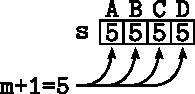
\includegraphics[scale=0.9]{quicksearch-1.pdf} 
		\end{figure}
	\item \textbf{Anpassen des Shiftarrays für vorkommende Zeichen 
		im Pattern} \\
		Das Pattern \verb!p! wird durchlaufen mit Index \verb!i!
		und \verb!m!$-$\verb!i! in das zutreffende Element vom
		Shiftarray eingetragen. Die kleine Zahl überwiegt!
		\begin{figure}[h!]
			\centering
			\hfill{} \hfill{}
			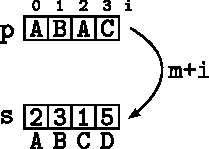
\includegraphics[scale=0.9]{quicksearch-2.pdf}
			\hfill{}
			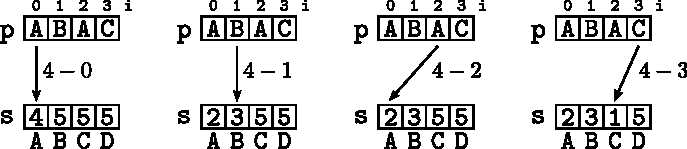
\includegraphics[scale=0.9]{quicksearch-3.pdf}
		\end{figure}
\end{enumerate}

\noindent
Nachdem das Shiftarray \verb!s! initialisert worden ist, kann mit der
Suche begonnen werden. Hierzu nimmt man das erste Zeichen des Patterns
\verb!p! und verlgeicht mit dem ersten Zeichen der Zeichenfolge \verb!a!.
Stimmt das Zeichen aus Pattern und Zeichenfolge überein, dann vergleicht
man das nächste Zeichen usw. Stimmen die Zeichen nicht überein, so
muss man in der Zeichenfolge \verb!a! vorrücken und zwar um so viele 
Stellen, wie es bis zum Ende des Pattern \verb!p! noch gibt $+1$.

\begin{figure}[h!]
	\centering
	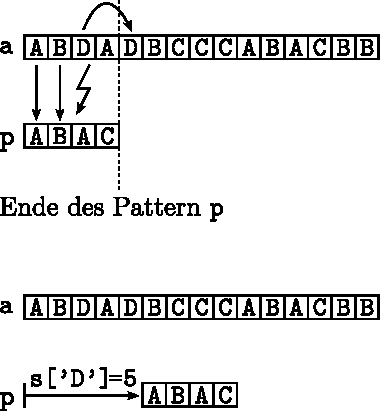
\includegraphics[scale=0.9]{quicksearch-7.pdf}
\end{figure}

\subsubsection{Source}
\lstinputlisting[title=Quicksearch in Java]{quicksearch.java}




		% Quicksearch		

\end{document}

